\section{DoublyLinked List} \label{sec:DoublyLinkedList_impl}

\subsection{Valg af datastruktur}

Faget \textit{Datastrukturer og Algoritmer} skulle indgå i projektet og derfor var det nødvendigt at vælge en datastruktur, som passede godt det til det vi lavede. 
I stedet for blot at anvende en præfabrikeret i \textit{STL}, ønskede vi at lave en datastruktur selv. 
Standard strukturen \textit{vektor} var en mulighed, men den blev valgt fra da en \textit{Doubly Linked List} (fremover benævnt DLL) er velegnet til at indsætte, fjerne og hente data fra front eller bag. 
Da der i projektet var brug for at indsætte og hente data ofte, faldt valget på denne datastruktur.

\subsection{Forklaring af Doubly Linked List}

En DLL er en udbygning af datastrukturen \textit{Linked List} og denne udbygning, har stedet for kun at have ét info felt til data og én next-pointer til det næste element i listen, har den også en previous-pointer. 
Med denne ekstra pointer, er det således muligt at gå frem og tilbage i listen, hvorimod en normal linked list kun kan gå frem. Klassen er implementeret som en template klasse, så alle simple typer kan bruges. I tilfældet at typen er kompleks, kan der implementeres overloads på equal-operatoren og >>.
Konceptet kan være lidt svært at forstå, men tænk på det som en analogi: Et tog. Programmøren gemmer altid det første knudepunkt på listen. 
Dette svarer til at være motoren i toget. Pointeren er koblingen, der sidder mellem vognene på toget. Hver gang toget tilføjer en vogn, bruger vi koblingen til at tilføje en ny vogn.

I Figur \ref{fig:nodes_cohe} er der vist et billede som viser hvordan tre noder er linket sammen.

\begin{figure}[ht]
\centering
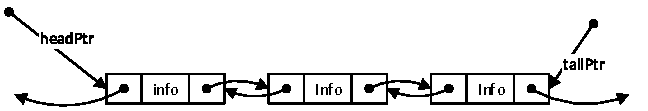
\includegraphics[width=\textwidth-5cm]{../fig/linkedNodes.pdf}
\caption{Sammenhængen mellem nodes.}
\label{fig:nodes_cohe}
\end{figure}

\clearpage

\subsection{HeadInsert}

I Listing \ref{lst:headInsert()} ses metoden til at indsætte data i DLL'en.

\lstinputlisting[linerange=headInsert0-headInsert1, label=lst:headInsert(), caption=Implementering af headInsert()]{../src/AutoGreenSem3/Devkit8000/autogreenbuild3/DoublyLinkedList.hpp}

Som det fremgår af Listing \ref{lst:headInsert()}, bliver headPtr og tailPtr sat til at pege på den nye node som er indsat, hvis der ikke er lavet nogen liste. I det tilfælde at en liste allerede er konstrueret, sætter metoden den nye node headPtr lig med noden lige før den. En DLL har også en tailInsert, som kan indsætte data i enden af listen efter næsten samme princip. 

\subsection{GetItemInList}
DLL'en holder også styr på, hvor mange elementer der er indsat. Således er der kontrol over hvor lang listen er, hvilket bruges internt i klassen, så det ikke kan lade sig gøre at slette en node på plads 7 hvis der kun er 4 noder i hele listen. Metoden for at få vist hvor mange elementer der findes i listen, ses i Listing \ref{lst:GetItemInList} 

\lstinputlisting[linerange=GetItems0-GetItems1, label=lst:GetItemInList, caption=Implementering af getItemInList()]{../src/AutoGreenSem3/Devkit8000/autogreenbuild3/DoublyLinkedList.hpp}

For at denne metode virker korrekt, er det meget vigtigt at alle metoder, der laver en mutation i strukturen, opdaterer den private variabel: itemsInList som beskrives i tabel \ref{table:DoublyLinkedList_attributter}, så den hele tiden passer med det, der bliver udført. Dvs. hvis noget tilføjes, skal der adderes én til variablen, modsat hvis der fjernes der noget skal der subtraheres én.
Det er også muligt at slette en node i en DLL via. metoden deleteAt(int place). Metoden kan ses i Listing \ref{lst:deleteAt()}. \clearpage



\subsection{DeleteAt}

Det er også muligt at slette en node i Doubly linked listen via. Metoden: deleteAt(int place). Metoden kan ses i tabel \ref{table:DoublyLinkedList_deleteAt}

\lstinputlisting[linerange=deleteAt0-deleteAt1, label=lst:deleteAt(), caption=Implementering af deleteAt(int place)]{../src/AutoGreenSem3/Devkit8000/autogreenbuild3/DoublyLinkedList.hpp}

For at give et bedre overblik over hvad der sker i koden ses i Figur \ref{fig:step1} og frem til \ref{fig:step4} en grafik, som beskriver hvordan det foregår i 4 steps.

\clearpage

Dette er et eksempel på en DLL, hvor 3 noder er sammensat. Node 2 ønskes fjernet fra DLL’en. 

\begin{figure}[ht]
\centering
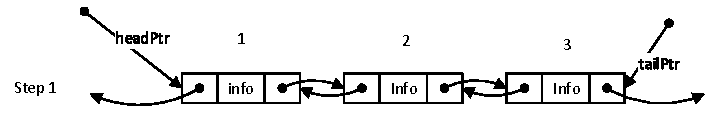
\includegraphics[width=\textwidth-5cm]{../fig/linkedNodStep1.pdf}
\caption{Tre noder, step 1.}
\label{fig:step1}
\end{figure}

Som det ses, er next-pointeren til node 1 flyttet, så den nu peger på node 3 og previous-pointeren fra node 3 peger nu på node 1. 

\begin{figure}[ht]
\centering
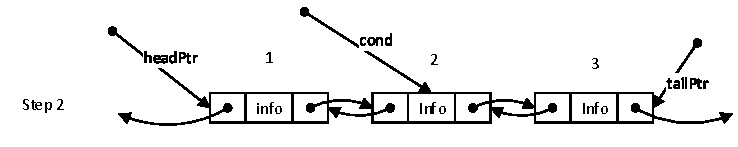
\includegraphics[width=\textwidth-5cm]{../fig/linkedNodStep2.pdf}
\caption{Ny pointer, step 2.}
\label{fig:step2}
\end{figure}


Der laves en ekstra pointer, som benævnes cond, og som sættes til at pege på node 2, således noden ikke mistes når step 3 flytter på pointere til node 1 og 2.

\begin{figure}[ht]
\centering
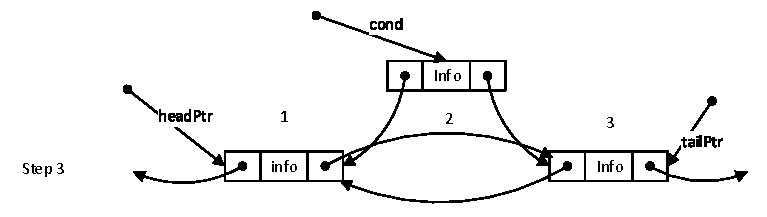
\includegraphics[width=\textwidth-5cm]{../fig/linkedNodStep3.pdf}
\caption{Flytning af pointere, step 3.}
\label{fig:step3}
\end{figure}

Dette betyder at node 2 nu er ude af systemet og kan slettes sikkert og uden at det ødelægger den listen. Efterfølgende er der kun node 1 og 3 tilbage og listen har nu fået fjernet node 2.

\begin{figure}[ht]
\centering
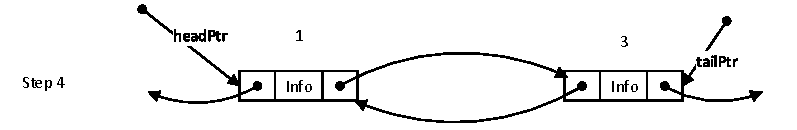
\includegraphics[width=\textwidth-5cm]{../fig/linkedNodStep4.pdf}
\caption{Sletning af node, step 3.}
\label{fig:step4}
\end{figure}

\subsection{PeekHead}

Metoden spørger efter det element som ligger gemt i fronten af listen. Metoden er særdeles vigtig, da det sikres det gemte materiale i listen kan hentes ud igen. Som der ses i metodesignaturen, returnerer metoden 1, hvis operationen gik godt og -1, hvis der var fejl. Metoden hvorpå der kan hentes elementer fra DLL'en kan ses i Figur \ref{lst:peekHead}.
\lstinputlisting[linerange=PeekHead0-PeekHead1, label=lst:peekHead, caption=Implementering af PeekHead.]{../src/AutoGreenSem3/Devkit8000/autogreenbuild3/DoublyLinkedList.hpp}